\chapter{Implementation Test} \label{secImpl}
In this chapter, a brief description of demonstration testing cases as well as test results is presented. To be more specifically, two test scenarios related with \emph{CommunicationStack} Java Card applet and simulated remote administrator server are designed. Also, the test cases demonstrating communication between Smart Home web server and Android application \emph{Smart Home App} are introduced.

\section{Javacard Applet and Remote Administrator Server Tests}
The aim of this testing scenario is to prove the reliability of applying Smart Card and Globalplatform standardized remote application/file management protocols to provide a secure dual authentication mechanism and messaging platform for other high-level applications. My Java Card Applet - \emph{CommunicationStack} together with correspondingly designed \emph{UTE} test cases are employed and build the testing environment. For reference, \emph{UTE} is introduced in section~\ref{secTS} together with other testing tools.

\subsection{\emph{UTE} Test Cases}

Two \emph{UTE} test cases are programmed. They are:
\begin{itemize}
\item \emph{Trigger Communication Channel with SMS}. In this test case, I simulate the open communication channel process between smart card and remote administrator server. This process is the cornerstone for a successful remote application management.
\item \emph{Secure Messaging.} After a successful identification between communication peers and creation of communication channel, in this test scenario, smart card and remote server are going to perform secure messaging. 
\end{itemize}

\subsubsection{Trigger Communication Channel with SMS} \label{secAppletTest1}
In this test suit, \emph{UTE} testing case acts as the remote administrator server and encapsulates information necessary for the construction of a secure Http channel in a \emph{TriggerPushSMS} object and sent this \emph{TriggerPushSMS} to target smart card applet using simulated GPRS connection. The structure of \emph{TriggerPushSMS}  is pictured in figure~\ref{fig:push-sms} and includes parameters which can be categorized as following:
\begin{figure}[!htb]
	\centering
	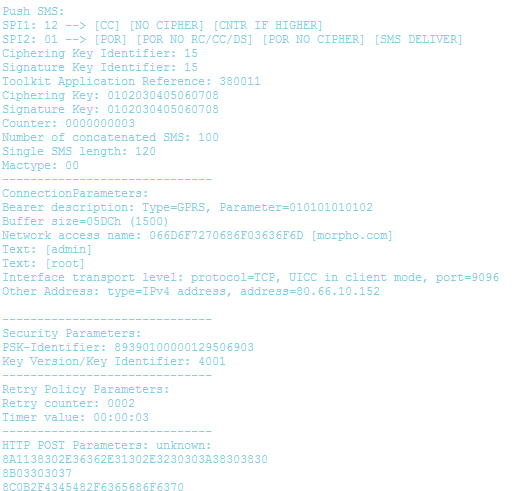
\includegraphics[width=1.0\textwidth]{Images/impl/push-sms.png}
		\caption{Screen-shot of Push Short Message including parameters which are necessary for the communication channel construction}
	\label{fig:push-sms}
\end{figure}
\begin{itemize}
\item \emph{Connection Parameters}, which includes network access name, bearer description and other parameters describing the simulated remote server.
\item \emph{Smart Card Keysets}, that consist of key identifiers as well as indicator used for the select of cipher keys and signature keys. As described in section~\ref{labelKeyManagement}, in order to retrieve a particular cipher key from Smart Card  key management system, information such as key identifier must be provided.
\item \emph{Http connection parameters}. Parameters such as retry counter, timeout values are included in this short message.
\end{itemize}
After a successful receiving and processing of aforementioned push \emph{TriggerPushSMS}, \emph{CommunicationStack} will preform TLS handshake with the remote server. 

The TLS \emph{client-hello} message is demonstrated by figure~\ref{fig:client-hello}. The version of TLS protocol, random number as well as proposed cipher suits are encapsulated.   The corresponding TLS \emph{server-hello} message is presented by figure~\ref{fig:server-hello} and in this demonstration case as shown cipher suit \emph{TLS\_PSK\_WITH\_NULL\_SHA256} is chosen. At last, the master key, shown in figure~\ref{fig:mk} is generated between remote server and card applet.

\begin{figure}[!htb]
	\centering
	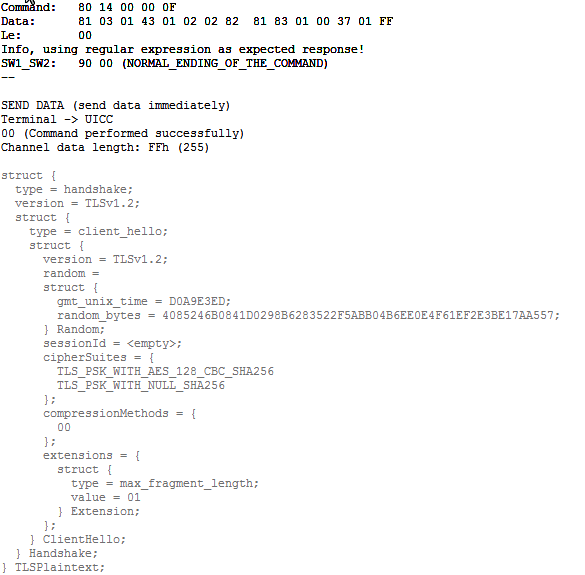
\includegraphics[width=1\textwidth]{Images/impl/client-hallo.png}
		\caption{Screen-shot of TLS client-hello-message sent by smart card applet}
	\label{fig:client-hello}
\end{figure}

\begin{figure}[!htb]
	\centering
	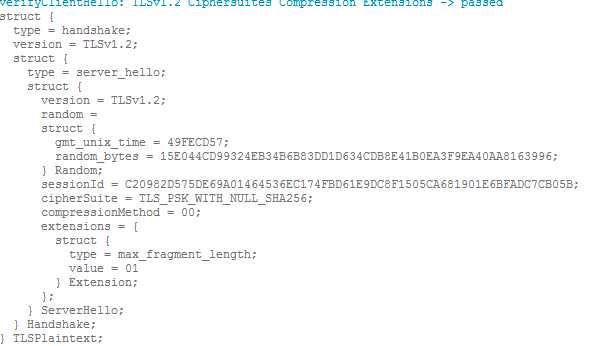
\includegraphics[width=1\textwidth]{Images/impl/ServerHallo.jpg}
		\caption{Screen-shot of TLS server-hello-message sent by remote server}
	\label{fig:server-hello}
\end{figure}

\begin{figure}[!htb]
	\centering
	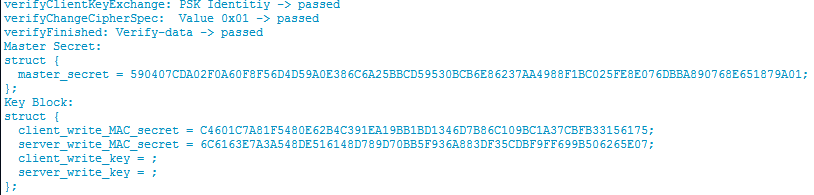
\includegraphics[width=1\textwidth]{Images/impl/master-key.png}
		\caption{Screen-shot of successful generation of master key between remote server and \emph{CommunicationStack} applet}
	\label{fig:mk}
\end{figure}


\subsubsection{Secure Messaging Exchanging}



Based on the in previous test created secure channel and Http Connection, in this test case, smart card applet and remote server perform secure message exchange using newly generated master key. 

\begin{figure}[!htb]
	\centering
	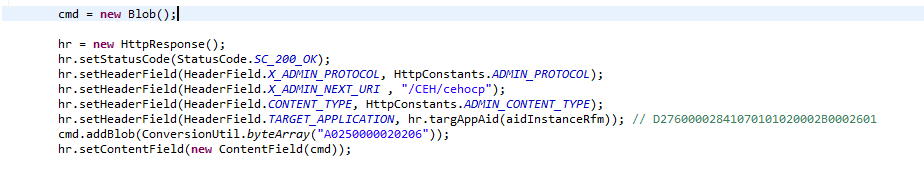
\includegraphics[width=1.1\textwidth]{q1.png}
		\caption{Screen-shot of Http message configuration in test case}
	\label{fig:q1}
\end{figure}

The \emph{UTE} test code snippet shown in figure~\ref{fig:q1} generates a Http response message using header defined in section~\ref{secHttpHeader} to the \emph{CommunicationStack} applet, whose AID is set as \emph{D27600002841070101020002B0002601}. The body of this message includes a command APDU, whose content is \emph{A0250000020206}.


\begin{figure}[!htb]
	\centering
	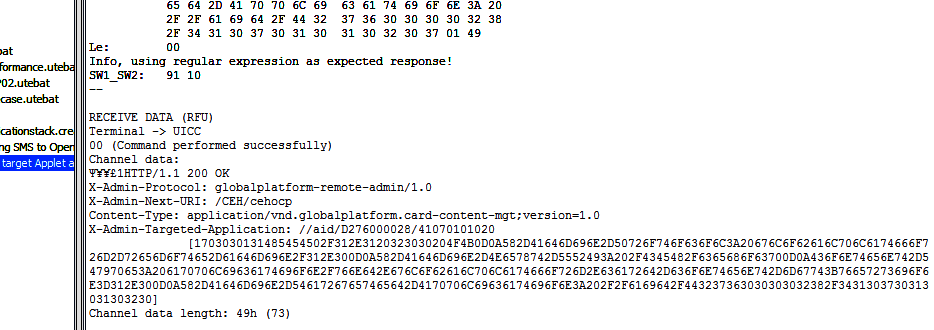
\includegraphics[width=1\textwidth]{q2.png}
		\caption{Screen-shot of Http message generated by simulated remote administrator server}
	\label{fig:q2}
\end{figure}

As illustrated in figure~\ref{fig:q2}, the simulated remote server successfully generated this Http response message and transmitted it to the Java Card applet.

After receiving this Http Message from remote server, my applet is able to retrieve the encapsulated command data, to be more precisely, as illustrated in figure~\ref{fig:remote1}, the command data \emph{A0250000020206} can be retrieved. Furthermore as shown in figure~\ref{fig:q3}, at the end of this testing scenario, remote server receives a Http message from \emph{CommunicationStack} applet and the content of this message is apparently secured, whose clear test is presented in figure~\ref{fig:q4}.
The Http header I applied in those test cases are compliant with the ones introduced in section~\ref{secHttpHeader}.


\begin{figure}[!htb]
	\centering
	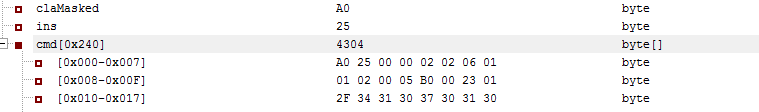
\includegraphics[width=1\textwidth]{Images/impl/cmd.png}
		\caption{Screen-shot of {cmd} Buffer in \emph{CommunicationStack} applet}
	\label{fig:remote1}
\end{figure}

\begin{figure}[!htb]
	\centering
	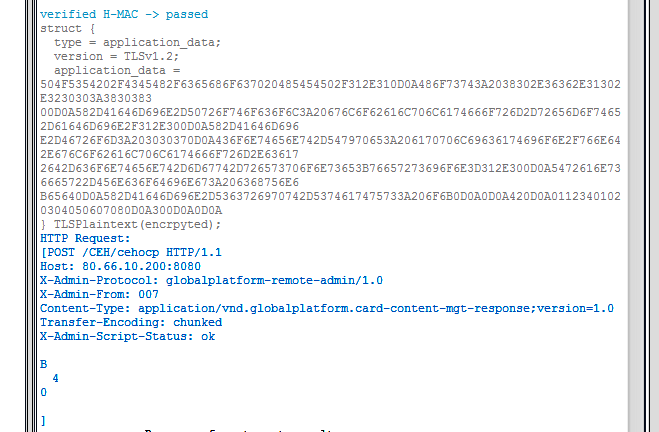
\includegraphics[width=1\textwidth]{q3.png}
		\caption{Screen-shot of Http message received by remote server}
	\label{fig:q3}
\end{figure}

\begin{figure}[!htb]
	\centering
	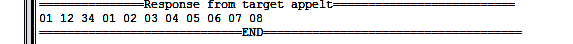
\includegraphics[width=1\textwidth]{q4.png}
		\caption{Screen-shot of translation of Http content of figure~\ref{fig:q3}}
	\label{fig:q4}
\end{figure}

\section{Android Application Tests}
In this section, how my Android application interacts with Smart Home web server as well as with smart card applet will be demonstrated.

\subsection{PIN Verification}

As already introduced, in order to use functionalities provided by \emph{Smart Home App}, phone holder must authenticate himself by inputing PIN for Android application. But after three times wrong PIN input as shown in figure~\ref{fig:sub1}, PIN will be locked as shown in figure~\ref{fig:sub2}. Only the Smart Home service provider can unblock the locked PIN. 
\begin{figure}[!htb]
\begin{minipage}{0.49\linewidth}
  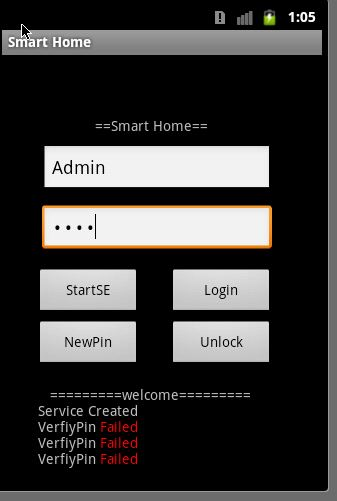
\includegraphics[width=0.8\linewidth]{Images/impl/3failed.jpg}
  \caption{Screen-shot of Wrong PIN input}
  \label{fig:sub1}
\end{minipage}
    \hfill
\begin{minipage}{0.49\linewidth}
  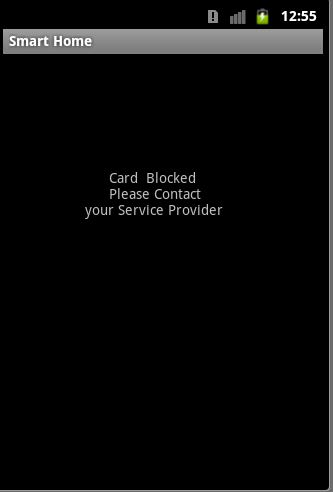
\includegraphics[width=0.8\linewidth]{Images/impl/UI3.jpg}
  \caption{Screen-shot of blocked PIN}
  \label{fig:sub2}
\end{minipage}
  \end{figure}

\subsection{Communication with Web Server}
After a successful identification, Android application user now can enjoy functions provided by Smart Home application, such as remote housing device management and querying historical data, as presented in following.

Moreover, as shown in figure~\ref{fig:housing-device}, house holder can select the name of housing device in the first drop-down menu and  choose associating functions from the second drop-down menu. To be more precisely, following housing devices and functions are simulated,
\begin{figure}[!htb]
	\centering
	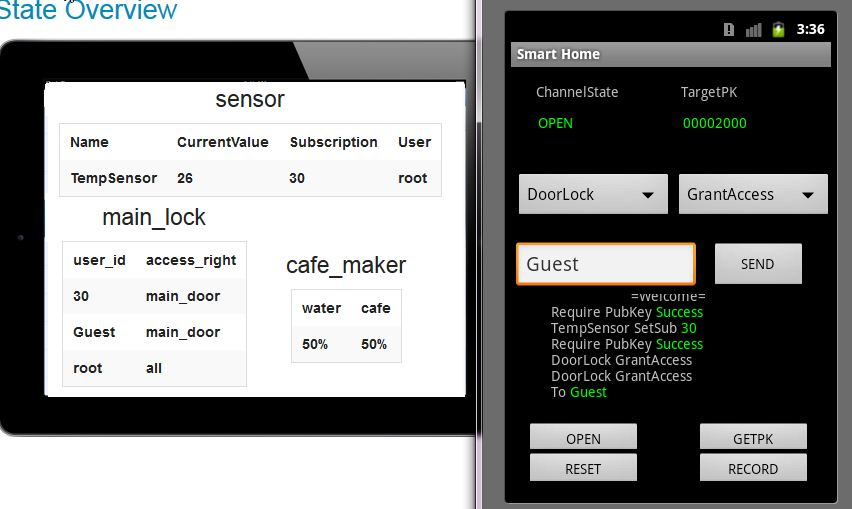
\includegraphics[width=1\textwidth]{Images/impl/housing-device.jpg}
		\caption{Using Android application remotely managing home devices}
	\label{fig:housing-device}
\end{figure}

\begin{itemize}
\item Temperature Sensor, which provides functions for getting current sensor value and setting subscription .
\item Coffee Maker,  which offers add water, add coffee and make coffee services.
\item Digital Door Lock, which can receive  \emph{openDoor}, \emph{closeDoor} and  \emph{grantAccessToOthers} commands.
\end{itemize}

Meanwhile the four buttons in the bottom of  \emph{Smart Home App} main screen as shown in figure~\ref{fig:housing-device} provide following functionalities,
\begin{itemize}
\item \emph{OPEN}, which is used to inform smart card to create secure channel with the remote administrator sever.
\item \emph{GETPK}, which is used to query public key of desired housing device selected  by the first drop-down menu.
\item \emph{RESET}, which is used to reset the current state of this Android application
\item \emph{RECORD}, which is used to achieve Smart Home historical records as shown in figure~\ref{fig:record-query}.

\end{itemize}

\begin{figure}[!htb]
	\centering
	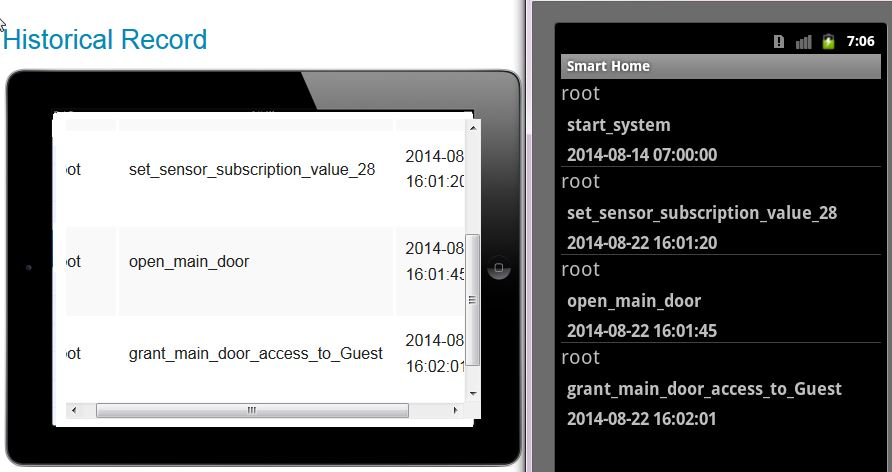
\includegraphics[width=1\textwidth]{Images/impl/record-query.jpg}
		\caption{Historical Record Overview}
	\label{fig:record-query}
\end{figure}

\section{Conclusion}
In conclusion, as the testing result shows, my proposal is practical and secure. The demonstration system is able to create secure connection between communication partners. The created communication channel is based on Http connection secured by TLS 1.2 standard. With the help of Morpho Smart Card OS and RAM/RFM standards from GlobalPlatform, my Java Card applet \emph{CommunicationStack} is capable of performing successful mutual identification as well as secure messaging with the remote administrator server. Moreover, all exchanged messages are well-formed and carefully encrypted. The demonstrated Smart Home takes care of the integrity of exchanged data, confidentiality of user credentials and at the same time provides traceability records.